% Каркас отчёта (<= 2 страницы). Компилятор Overleaf: pdfLaTeX (по умолчанию).
% Графики и таблица генерируются командой `pixi run figures` в репозитории (report/make_figures.py).
\documentclass[10pt,a4paper]{article}
\usepackage[T2A]{fontenc}
\usepackage[utf8]{inputenc}
\usepackage[russian,english]{babel}
\usepackage[a4paper,margin=1.8cm]{geometry}
\usepackage{graphicx,booktabs,multirow,amsmath,caption}
\usepackage[hidelinks]{hyperref}
\usepackage[font=small]{subcaption}
\captionsetup{font=small,skip=3pt}
\setlength{\textfloatsep}{8pt}
\setlength{\parskip}{0pt}
\graphicspath{{figures/}}
% generated by report/make_figures.py
\newcommand{\orbruns}{garden: 1.38/1.53/2.55; campus: 2.41/2.84/3.13; park: 1.78/1.99/2.02}


\title{\vspace{-1.5cm}Сравнение методов VIO на колёсном роботе (ROVER)}
\author{TODO: ФИО, группа}
\date{}

\begin{document}
\selectlanguage{russian}
\maketitle
\vspace{-1cm}

\section*{Методы}
% TODO: OpenVINS [1] (фильтр MSCKF, 2020), ORB-SLAM3 [2] (оптимизация по ключевым кадрам, 2021),
% DBA-Fusion [3] (обучаемый плотный BA + граф факторов с IMU, 2024). Суть, вклад, почему выбраны.

\section*{Данные и метрики}
% TODO: ROVER [4], камера T265 (левый fisheye) + IMU, GT — призма тахеометра (~2 Гц, только позиция).
% APE после SE(3)-выравнивания (Umeyama), RPE на отрезках 10 м, evo [5]; Sim(3) и масштаб s* — для анализа.

\section*{Результаты}

\begin{table}[h]
\centering\small
\caption{Ошибки на ROVER. APE~--- RMSE абсолютной ошибки положения после выравнивания SE(3) или Sim(3);
$s^*$~--- масштаб, подобранный Sim(3) ($s^*>1$: метод недооценил путь); RPE~--- RMSE относительной ошибки
на отрезках 10~м (только трансляция). Для ORB-SLAM3 медианный по APE из трёх прогонов
(\orbruns~м).}
\label{tab:res}
% generated by report/make_figures.py -- do not edit by hand
\begin{tabular}{llcccc}
\toprule
Seq. & Method & APE SE(3), m & APE Sim(3), m & $s^*$ & RPE@10\,m, m \\
\midrule
\multirow{3}{*}{garden, 121 m} & OpenVINS & 0.84 & \textbf{0.60} & 0.90 & \textbf{0.98} \\
 & ORB-SLAM3 & 1.53 & 1.16 & 1.24 & 2.51 \\
 & DBA-Fusion & \textbf{0.78} & 0.72 & 1.06 & 1.02 \\
\midrule
\multirow{3}{*}{campus, 150 m} & OpenVINS & 1.83 & 1.64 & 0.89 & 1.11 \\
 & ORB-SLAM3 & 2.84 & 2.25 & 1.37 & 4.51 \\
 & DBA-Fusion & \textbf{0.64} & \textbf{0.56} & 1.05 & \textbf{0.77} \\
\midrule
\multirow{3}{*}{park, 164 m} & OpenVINS & \textbf{1.68} & 1.64 & 0.96 & \textbf{1.42} \\
 & ORB-SLAM3 & 1.99 & \textbf{0.76} & 1.30 & 2.67 \\
 & DBA-Fusion & 5.71 & 5.16 & 0.71 & 3.37 \\
\bottomrule
\end{tabular}

\end{table}

\begin{figure}[h]
\centering
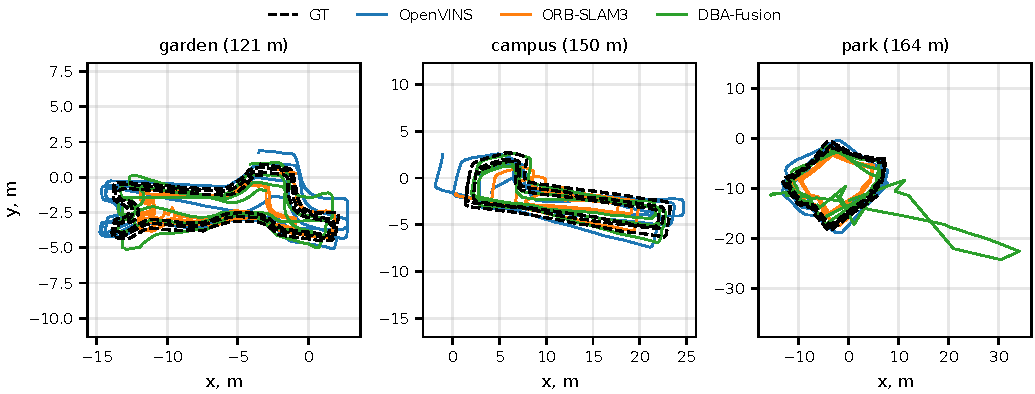
\includegraphics[width=\textwidth]{traj_xy.pdf}
\caption{Вид сверху после SE(3)-выравнивания. GT~--- положение призмы тахеометра.}
\label{fig:traj}
\end{figure}

% Можно поставить рядом с текстом выводов (половина ширины):
\begin{figure}[h]
\centering
\begin{minipage}[t]{0.49\textwidth}\vspace{0pt}
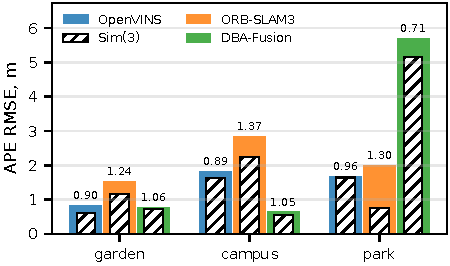
\includegraphics[width=\linewidth]{scale_se3_sim3.pdf}
\end{minipage}\hfill
\begin{minipage}[t]{0.48\textwidth}\vspace{0pt}
\caption{APE при выравнивании SE(3) (цветные столбцы) и Sim(3) (штриховка); над столбцом~--- $s^*$.
Разрыв между ними~--- вклад ошибки масштаба.}
\label{fig:scale}
\end{minipage}
\end{figure}

\begin{figure}[h]
\centering
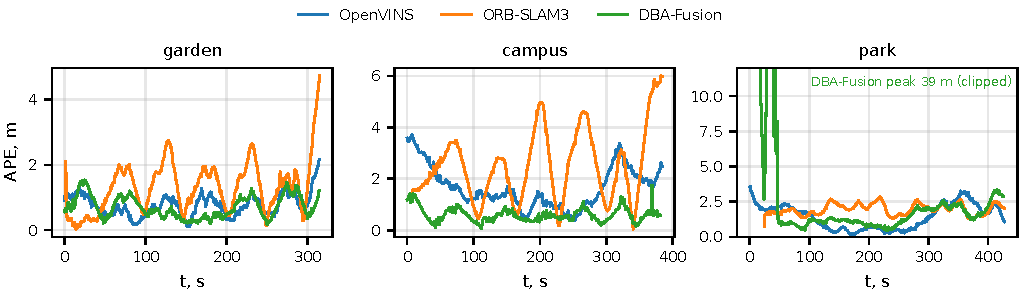
\includegraphics[width=\textwidth]{ape_time.pdf}
\caption{APE во времени (выравнивание SE(3), как в табл.~\ref{tab:res}). На park у DBA-Fusion сбой первых $\sim$60~с после инициализации (ось обрезана).}
\label{fig:ape}
\end{figure}

% Опционально, если хватит места:
% \begin{figure}[h]
% \centering
% 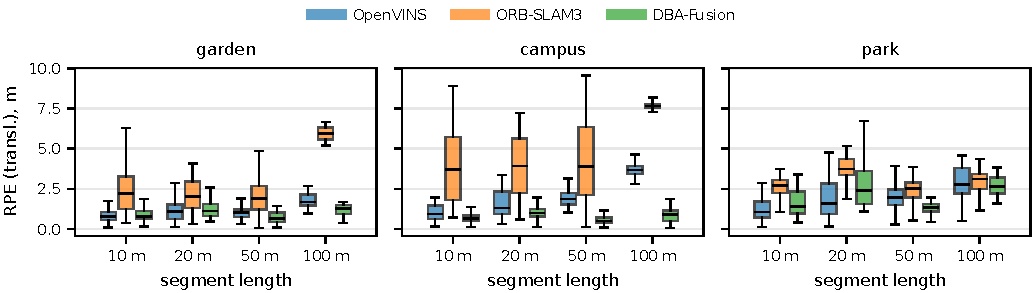
\includegraphics[width=\textwidth]{rpe_segments.pdf}
% \caption{RPE (трансляция) на отрезках 10--100~м.}
% \label{fig:rpe}
% \end{figure}

\section*{Выводы}
% TODO

\begin{thebibliography}{9}\small
\setlength{\itemsep}{0pt}
\bibitem{ov} P.~Geneva et al. OpenVINS: A Research Platform for Visual-Inertial Estimation. ICRA, 2020.
\bibitem{orb} C.~Campos et al. ORB-SLAM3: An Accurate Open-Source Library for Visual, Visual-Inertial and Multi-Map SLAM. IEEE T-RO 37(6), 2021.
\bibitem{dbaf} Y.~Zhou et al. DBA-Fusion: Tightly Integrating Deep Dense Visual Bundle Adjustment with Multiple Sensors for Large-Scale Localization and Mapping. IEEE RA-L, 2024. arXiv:2403.13714.
\bibitem{rover} ROVER dataset. TODO: точная ссылка на статью/страницу датасета.
\bibitem{evo} M.~Grupp. evo: Python package for the evaluation of odometry and SLAM. \url{https://github.com/MichaelGrupp/evo}, 2017.
\bibitem{repo} Код и инструкции по воспроизведению: \url{https://github.com/yahigz/robotics-vio-test}.
\end{thebibliography}

\end{document}
